%!TEX root = ../main.tex
\doublespacing
\chapter{Future Work and Conclusions}
\label{chap:future}
The principal goals of this thesis were to observe solar radio emission at the highest temporal, spectral and spatial resolutions to date. Firstly, the REAL-time Transient Acquisition backend (REALTA) was developed and installed at I-LOFAR to record the raw voltages from the station at $5.12 \mu$s temporal resolution. This work was published in \textit{Astronomy and Astrophysics} as \cite{Murphy2021b}
Secondly, a new technique was implemented for the first time to directly measure the size of radio bursts from their interferometric visibilities. This work was presented in Chapter \ref{chap:measuring_source_sizes} and was published in \textit{Astronomy and Astrophysics} as \cite{Murphy2021}. This technique was utilised to determine the size and shape of 29 type III bursts that were compared with predictions from state-of-the-art scattering simulations.
In this chapter I highlight some future work that could be built upon the research presented in this thesis to further advance the knowledge of radio wave generation and propagation in the solar corona. I discuss the possibility of observing radio bursts with 5~ns temporal resolution using the Transient Buffer Boards (TBBs) from I-LOFAR. Next I consider the use of machine learning algorithms to automatically detect and classify solar radio bursts recorded with I-LOFAR and REALTA. I then discuss the necessity for the development of a calibration and imaging pipeline for solar interferometry. I also outline further work that is necessary to bridge the gap between modern observations and computer simulations. This is underscored by the need for a statistical analysis of type III and type IIIb radio bursts, particular in the context of the most recent theories of spectral fine structure generation due to Langmuir wave modulation. Finally, I draw this thesis to a close with some concluding remarks.

\section{Primary Scientific Objectives}
The research that has been presented in this thesis has contributed to our knowledge of solar radio emission at low frequencies. The extent to which radio wave propagation effects distort the original shape of a radio burst has been explored. Work undertaken during this thesis has also resulted in a new facility to record and analyse radio emission using I-LOFAR. REALTA can be used to record radio observations at 5.12~$\mu$s temporal resolution. A new technique for measuring burst sizes from complex visibility data was also developed over the course of this work. Below I summarise the results from this thesis. 

\subsection{Observing Radio Bursts at the Highest Temporal Resolutions.}
The first objective of this thesis was to record the high time resolution, raw voltages from I-LOFAR to observe solar radio bursts.
In order to do this, a dedicated backend to record, store and analyse the data was necessary. Chapter \ref{chap:REALTA} outlines the development of the REALtime Transient Acquisition backend (REALTA) to serve this purpose. The seven node computer cluster receives data from I-LOFAR along a 10~Gbps fibre optic cable in four data ``lanes". After data has been recorded to disk, one of a number of processing pipelines can be run including those for solar radio observations, pulsars, FRBs, RRATs, Jovian emission and SETI. Some of the first solar radio bursts observed with I-LOFAR and REALTA are shown in Chapter \ref{chap:REALTA}. REALTA allows for high temporal resolution observations of short duration solar radio bursts such as S-bursts and can be used to analyse short duration pulsations in radio bursts. Information gained from such observations can be used to remotely determine the physics of the solar corona \citep{Morosan2015, Clarke2019} and can give insight into magnetohydrodynamic oscillations in the corona \citep{Carley2019}. This work was published in \textit{Astronomy and Astrophysics} as \cite{Murphy2021b}. Some other first results from REALTA are given below.
\subsubsection{Pulsars}

% ---Pulsar justification---
International LOFAR stations are ideal instruments to observe radio pulsars, particularly at frequencies between 100~MHz and 200~MHz \citep{Stappers2011, Bilous2014, Noutsos2015}. Furthermore, the large fractional bandwidth of an international LOFAR station can offer new insight to the spectral variability of giant pulses from the Crab Nebula. Many international stations regularly participate in pulsar studies \citep[for example,][]{Mereghetti2016, Bondonneau2017, Hermsen2018, Donner2019}, while pulsar observations with LOFAR core stations \citep[for example,][]{Bilous2014, Bilous2020} are also common. Recent observations with the Polish international stations include those by \cite{Blaszkiewicz2020}. 

To date, over 50 different pulsars have been observed with I-LOFAR using REALTA. Figure \ref{fig:pulsar-pc1} shows a sample of 19 pulsars which were observed, each for 6 minutes, on the 4th and 5th of March 2020, processed using the methods discussed in section \ref{sec:pulsarproc}. In addition, as a result of regular timing campaigns of these sources, a number of targets have been studied in more depth, the Crab Nebula being the prime example. 
\begin{figure*}[t]
    \centering
    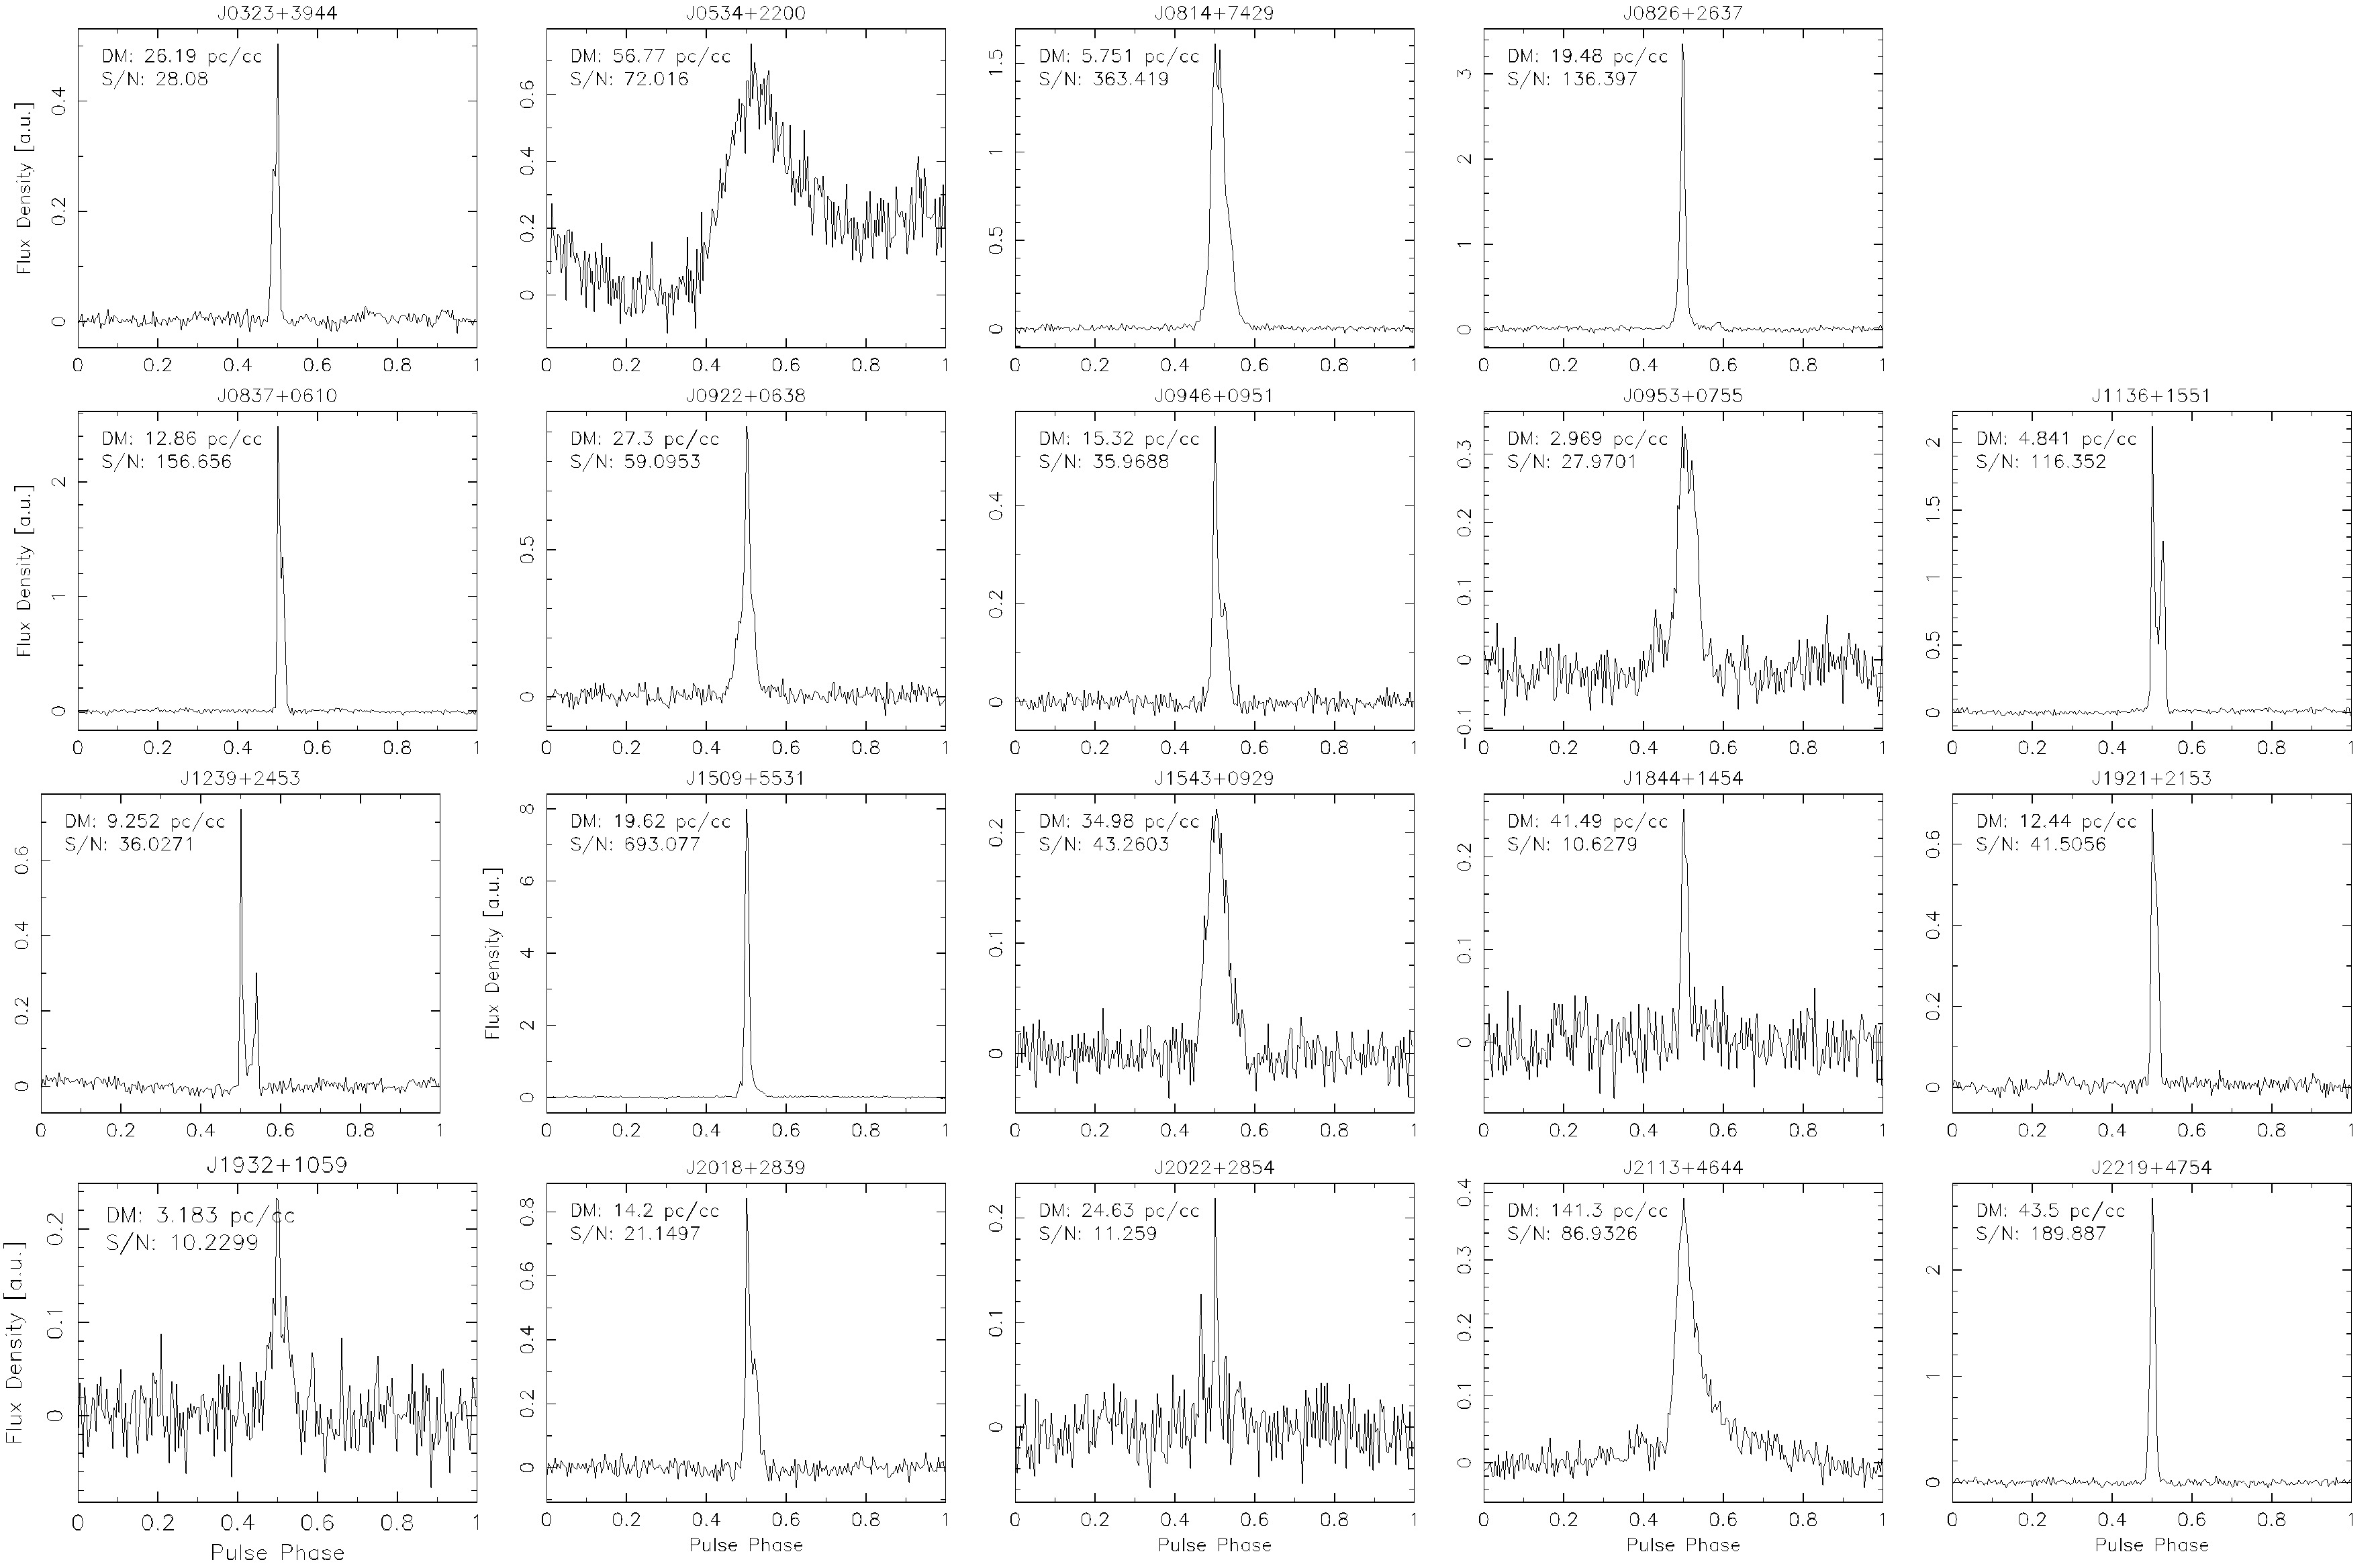
\includegraphics[width=0.92\textwidth]{psr_profiles.jpg}
    \caption[Sample of 19 pulsars observed with I-LOFAR and REALqTA.]{Sample of 19 pulsars observed with I-LOFAR and REALTA. Each of these observations is 6 minutes in duration and were taken on 4--5 March 2020 using the HBA antennas (\SIrange{110}{190}{\mega \hertz}). The data were processed using the method described in section \ref{sec:pulsarproc} and plotted using \texttt{PSRCHIVE}. The x-axis in each plot is the pulse phase in radians, while the y-axis is flux density in arbitrary units.}
    \label{fig:pulsar-pc1}
\end{figure*}
While the recording and timing of folded profiles of the Crab pulsar are of interest for studying the interior structure of the neutron star via its glitches \citep{Lyne2015} and variability due to scattering and echo events, it also frequently emits so-called `giant pulses' \citep{Meyers2017}. These giant pulses have fluences that vary from hundreds of Jy\,ms to tens of thousands of Jy\,ms. These pulses can be studied to analyse their scintillation, scattering, and brightness distributions.

One such example of these giant pulses can be seen in an observation taken of the Crab pulsar with I-LOFAR on 30 June 2020. The observation was processed using the previously described methodology (section \ref{sec:baseproc}, section \ref{sec:pulsarproc}) on REALTA and a short segment of the observation is shown in Figure \ref{fig:giant_pulse}. The figure is made from Stokes I data, where each channel has a bandwidth of 24~kHz and an underlying time resolution of 40.96~$\mu$s (though it has been averaged using a median filter for this plot). There were $\sim 1300$ giant pulse candidates detected in the 30 minute observation. Using a rate of $\sim 0.7$ giant pulses per second, we determine there are $\sim 20$ giant pulses visible in the dynamic spectrum in the left panel of Figure \ref{fig:giant_pulse}. Other structure in the left panel of Figure \ref{fig:giant_pulse} includes some ionospheric scintillation and RFI. This time segment is mostly of interest due to one rare, extremely bright, giant pulse, which is re-plotted in the right panel of Figure \ref{fig:giant_pulse} where it has been corrected for dispersion effects. Initial analysis using the radiometer equation indicates a specific fluence of $\sim 200$~kJy~ms across the observed bandwidth which may be the brightest pulse ever observed for this pulsar at these frequencies \citep{Karuppusamy2012,Meyers2017,VanLeeuwen2020}.

As of May 2021, over 80 hours of observations of the Crab pulsar have been captured by REALTA. Initial analysis of this data set, focusing on a four hour observation from March of 2020, has been performed and gives results that are similar to that of other low-frequency instruments. The giant pulses were found to form a fluence distribution with a power-law fit of $\alpha = -2.86~\pm~0.07$, similar to that of other low frequency instruments \citep{Meyers2017}, but steeper than the results at Jodrell Bank \citep{Mickaliger2017}. Similarly, an initial investigation of the spectral behaviour of the scattering timescale of the brightest pulses appeared to follow a power law of $\alpha = -3.7 \pm 0.5$, in agreement with other instruments \citep{Driessen2019}. Future work includes planning to integrate a CLEAN-based de-convolution \citep[see][]{Bhat2003} of the pulse shapes to better describe the scattering and dispersion measure variations of single pulses over time, the effects of which are entangled \citep{McKee2018}, especially at lower frequencies.

\begin{figure}
    \centering
    \includegraphics[width=\columnwidth]{quickcrab.png}
    \caption[Observation of the Crab Pulsar performed on 30 June 2020.]{Observation of the Crab Pulsar performed on 30 June 2020, (left) without incoherent dedispersion and (right) with incoherent dedispersion. The plot on the left contains several giant pulses and both temporally- and spectrally-variable ionospheric scintillation.  The plot on the right focuses on the brightest pulse in the group, which is the brightest pulse observed from the Crab Pulsar with I--LOFAR to date. Here data were processed to channel bandwidths of 24~kHz, resulting in a sampling rate of 40.96$\mu$s. The data were time integrated to a temporal resolution of 1.31~ms prior to plotting.}
    \label{fig:giant_pulse}
\end{figure}

\subsubsection{Rotating radio transients}\label{sec:rratsurvey}
Rotating radio transients (RRATs) are a class of neutron star that were discovered through detecting single, bright pulses rather than via periodicity searches. If a sufficient number of pulses is detected within a short observing window, it is possible to determine the underlying period of the neutron star through brute force methods, after which the times of arrival of these pulses can be used to time the sources like any other pulsar \citep{Keane2011}. While the LOFAR core has blindly detected several RRATs during the LOFAR Tied Array All Sky survey \citep[LOTAAS][]{Sanidas2019, Michilli2020, Tan2020}, and through targeted follow-up observations of sources detected with the Green Bank Telescope \citep{Karako-Argaman2015}, there has not been a major undertaking to time these sources with the LOFAR instruments, using the core or international stations.
\begin{figure*}[t]
    \centering
    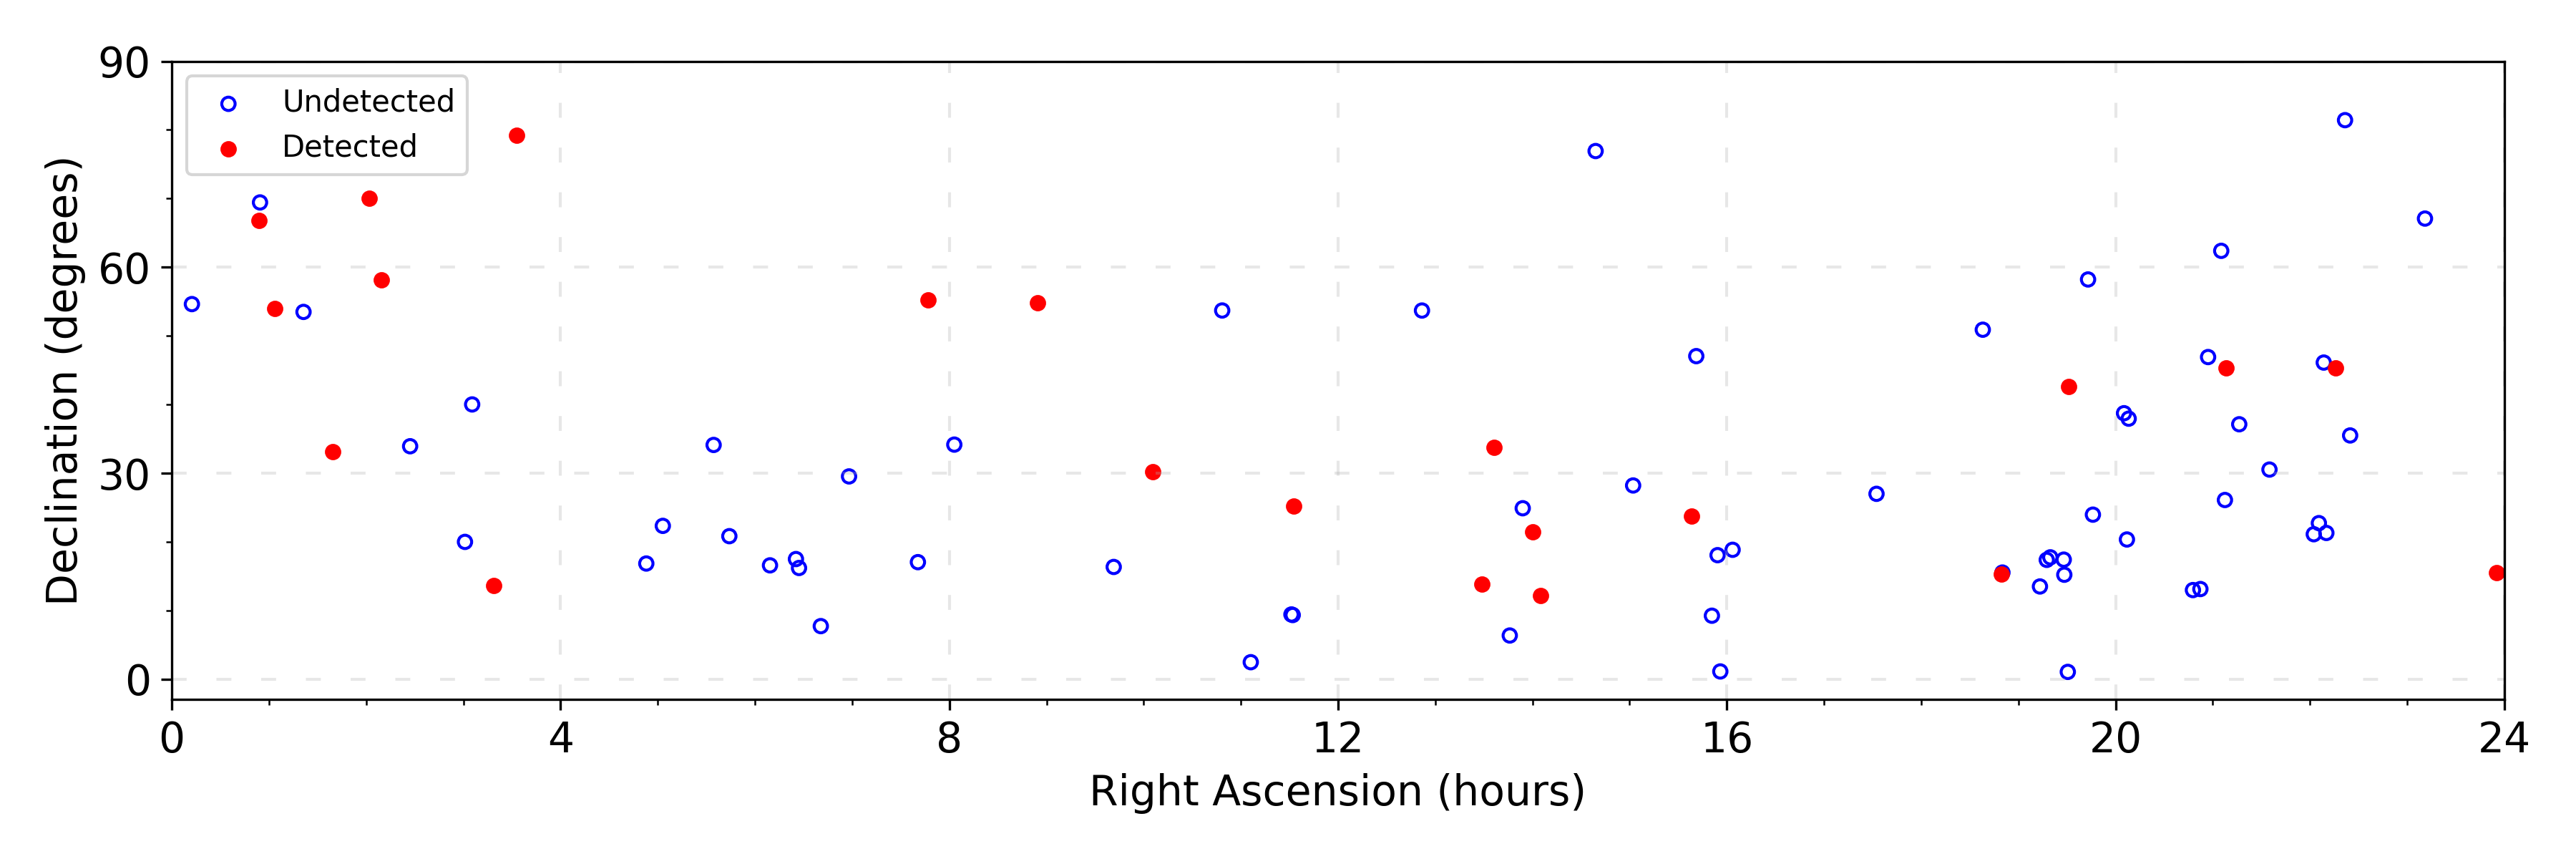
\includegraphics[width=0.92\textwidth]{rrat_observed.png}
    \caption[Overview of the sky positions of RRATs observed during RRAT census.]{Overview of the sky positions of the RRATs observed during the census discussed in section \ref{sec:rratsurvey} as of May 2021. Filled red dots indicate sources that have been observed and detected with either single pulses or periodic emission while blue circles indicate sources that were observed but not detected in I-LOFAR data.}
    \label{fig:rrat-pc1}
\end{figure*}
However, the full-sky sensitivity and fractional bandwidth of a single international LOFAR station makes it the perfect candidate to perform follow-up observations of some of the brighter RRAT candidates identified by all-sky monitoring instruments such as the Big Scanning Array of Lebedev Physical Institute (BSA LPI) and the Canadian Hydrogen Intensity Mapping Experiment \citep[CHIME;][]{Amiri2018}. Follow-up observations of these candidates are useful to (a) determine the rotational characteristics of the stars through phase-coherent follow-up timing; and to (b) perform source characterisation from examining stars with broad spectral coverage.

Between July 2020 and May 2021, a 500 hour observing campaign has been undertaken to observe a diverse set of RRATs from the RRatalog\footnote{\hyperref[RRatalog]{http://astro.phys.wvu.edu/rratalog/}}, the CHIME-FRB Galactic sources database\footnote{\hyperref[CHIME-FRB Galactic Sources]{https://www.chime-frb.ca/galactic}}, and the BSA LPI Transients Catalogue\footnote{\hyperref[BSA LPI Transients Catalogue]{https://bsa-analytics.prao.ru/en/transients/rrat/}}, with a focus on sources that as yet do not have well defined periods. An overview of the sources observed and detected by this census can be seen in Figure \ref{fig:rrat-pc1}. This campaign has so far resulted in the discovery of rotation periods for two sources which were previously unknown, periodic detection of a further two sources that have not been previously detected at LOFAR frequencies and the determination of coherent timing solutions for thirteen other sources. These results will be discussed in detail in a future paper (McKenna et al. in prep).%\citep{McKenna2021}.


\subsubsection{Fast radio bursts}
Since their discovery in 2007 by \citeauthor{Lorimer2007}, fast radio bursts (FRBs) have been of keen interest to radio astronomers across the globe. While blind searches with multiple telescopes have helped push the lower bounds of their emission frequencies down year on year, the detection of numerous repeating FRBs by the CHIME-FRB collaboration \citep{CHIME2019} has accelerated this process in recent months. Searches for FRBs with LOFAR include those by \cite{Karastergiou2015} and \cite{TerVeen2019}, for example.

One particular repeating FRB, FRB 20180916B (`R3') has been found to have a period of $16.35\pm 0.15$ days, with an activity window of 5 days \citep{Amiri2020}, and has been detected with the LOFAR core \citep{Pastor-Marazuela2020, Pleunis2021}. Prior to this, I-LOFAR and REALTA were used as a part of a 70 hour campaign to observe R3 during its activity phase and attempt to see emission at previously unseen frequencies. However, no significant pulse candidates were detected during this campaign. For further results and observations of other FRB sources see McKenna et al. (in prep).



\subsubsection{Jovian auroral radio emission}

%\begin{figure}
\begin{figure*}
    \centering
%       \includegraphics[width=\columnwidth]{Jupiter_Io_IE613.png}
        \includegraphics[width=\columnwidth]{Jupiter_Io_IE613.png}              
    \caption[Observation of a Jovian Decametric emission produced by the Io-Jupiter interaction.]{Observation of a Jovian Decametric emission produced by the Io-Jupiter interaction. Panel (a) shows Stokes I (in dB above background). Panel (b) displays Stokes V (in arbitrary units). The resolution is $84$~ms per $12.2$~kHz. The emission displays a strong negative value in Stokes V, which means a strong right-hand circular polarization. Panels (c) and (d) show respectively a $60$~s and $10$~s zoom-in of panel (a) (Stokes I), processed with the highest resolution available for this observation ($81.92$~$\mu$s per $12.2$~kHz). Millisecond drifting bursts are visible panel (d).}
    \label{fig:io-stokesI}
\end{figure*}


%After solar radio bursts, Jupiter's decametric emission (DAM) is the most intense radio emission in our solar system.  the Jovian DAM extends above the ionospheric cutoff frequency to a maximum of $\approx$ 40~MHz, and have been observed from the ground since the 1950s \citep{Burke1955}.
%Jupiter's decametric emission (DAM) has been observed from the ground since the 1950s \citep{Burke1955}. 
Decametric radio emission (DAM), the strongest component of Jovian auroral radiation, was discovered in 1955 by \cite{Burke1955}, with part of this emission controlled by the Io-Jupiter interaction \citep{Bigg1964}. The source of this radio emission is known to be due to the electron cyclotron maser instability (ECMI) in the Jovian magnetosphere, which occurs when a circularly polarised wave resonates with the gyration of electrons with relativistic energies \citep{Wu1979,Wu1985,Zarka1998, Treumann2006,Louarn2017GRL}. The ECMI amplifies the wave on the extraordinary R-X mode which can escape the source and propagate in free space as a radio wave, at a frequency very close to the local electron cyclotron frequency, which is proportional to the local magnetic field amplitude. Jovian DAM emissions are the only planetary radio emissions visible from the ground, since part of the DAM is emitted at a frequency above the ionospheric cutoff frequency ($\gtrsim 10$~MHz). BF observations of Jovian DAM using the LOFAR core stations have been used to test the sensitivity of LOFAR to exoplanetary radio emissions \citep{Turner2019, Turner2021}.

%On 13 October 2020, I-LOFAR detected observed Jovian DAM emission from 17:41:30 to 18:00:00 UTC. The Stokes I data from this observation is shown in Figure \ref{fig:io-stokesI} panels a and b while Stokes V for the period 17:47:00 - 17:57:00 UTC is shown in Figure \ref{fig:io-stokesI} panel c. Given this is Jovian DAM emission, the magnetic field of Jupiter can be probed through the relationship $\nu_{\rm MHz} = 2.8 B_{G}$. This gives a first order estimation of Jovian magnetic field, for which we cannot infer an altitude without a magnetospheric model, from $\approx 8$\textendash$11$ G ($22$\textendash $31$ MHz) as the electrons traverse along magnetic field lines in the magnetosphere. In order to know the exact position of the sources, it is necessary to make interferometric measurements with several LOFAR stations. \par

On 8 June 2021, I-LOFAR observed Jovian DAM emission produced by the Io-Jupiter interaction, from 04:10 to 05:30 UTC. The Stokes I and V data from this observation are shown in Figure \ref{fig:io-stokesI}a-b. An arc shape emission with a high intensity is observed between $\sim 04$:$55$ and $05$:$30$ (corresponding to the main Io-DAM emission), preceded by emissions with lower intensity starting at $\sim 04$:$10$ (corresponding to secondary Io-emissions). Looking at both the shape of the emission and its polarization (strong negative Stokes V value, corresponding to a right-handed circular polarization), we can determine that this emission is an Io-B emission \citep[coming from the north-dawn side of Jupiter, see][for example]{Marques2017}.

Moreover, we have with I-LOFAR access to very high temporal and frequency resolution, of which an example is shown Figure \ref{fig:io-stokesI}c,d ($81.92$~$\mu$s per $12.2$~kHz). This will allow us to study the microphysics of the Jovian decametric emissions, for example the millisecond bursts visible Figure \ref{fig:io-stokesI}d with a drifting feature in frequency with time ($\sim 25$-$30$~MHz). These millisecond drifts are thought to be electron bunches propagating along the magnetic field lines and can reveal both the energy of the resonant electrons as well as the potential drops (if present) along these fields lines \citep{Hess2007, Hess2009}. The high-resolution capability will also enable constraints to be placed on the position and movement of the sources, by interferometric measurements with several LOFAR stations, as well as the characteristics of the emission (for example, thickness and opening of the emission beam). Finally, I-LOFAR, combined with REALTA, is equipped to join the other LOFAR stations in the ground radio observation campaigns in support of the Jupiter space missions, both current (Juno\footnote{Such as the Juno Ground Radio Observation Support \hyperref[Juno]{https://maser.lesia.obspm.fr/task-1-data-collections/juno-ground-radio/}}) and future (JUICE, Europa-clipper).

%One could note that no such intense emission has been observed by the Nan\c{c}ay Decametric Array \citep[NDA;][]{Boischot1980} during the same time period and frequency range, which demonstrates the ability of I-LOFAR to observe high-time resolution low-frequency radio emissions from the Jovian magnetosphere (with REALTA to process the data), which are not detectable by other low-frequency radio telescopes. During this observation, Jupiter was not ideally placed in the sky, reaching a maximum of 11$^{\circ}$ in elevation. Since the sensitivity increases with the target elevation, observations of Jupiter at a higher elevation will give a higher Signal-to-Noise Ratio. Under favourable conditions, Jupiter can reach $\sim$ \textbf{58 degrees elevation for example, at opposition in December 2024}. Using a Hamaker beam model from \texttt{dreambeam} \cite{Carozzi2016}, we estimate a 95\% reduction in sensitivity at the currently observed elevation.\par
%The I-LOFAR LBA is 40 times more sensitive than the NDA \citep{Clarke2014}, and so it is not surprising that the NDA did not detect this particular DAM emission.

%the microphysics of these emissions (such as the frequency drift, the possibility of distinguishing multiple emissions).


\subsubsection{SETI}
International LOFAR stations such as I-LOFAR have very broad fields of view, particularly at frequencies less than 150~MHz \citep{VanHaarlem2013}. This, coupled with the ability to channelise data to bandwidths $\lesssim 1$~Hz, are favourable characteristics in SETI research.
BL is conducting one of the most sensitive, comprehensive, and intensive searches for technosignatures on other worlds across a large fraction of the electromagnetic spectrum \citep{Worden2017}. Targets of the BL program include one million nearby stars, one hundred nearby galaxies, the entire Galactic plane, and exotic astrophysical objects \citep[see][for detail]{Isaacson2017}. \cite{Gajjar2019} provides the current status of these observing campaigns, as well as listing a number of collaborative observing facilities that are working alongside BL for carrying out these sensitive studies. The BL program is collaborating with two of the international LOFAR stations: I-LOFAR and LOFAR-SE, which is located at Onsala (Sweden), to complement searches towards the above-mentioned BL targets at lower radio frequencies. Details of the dedicated hardware deployed at I-LOFAR is discussed in section \ref{sect:pipeline_SETI}. First-light observations were conducted with these BL nodes on 19 November 2020 towards PSR B1919+21 to validate the BL recording and conversion pipelines.
Recently, we also conducted observations of PSR B2217+47 on 21 April 2021 using the BL nodes for further pipeline development. Baseband data in the GUPPI format were converted to two different temporal and spectral resolution total intensity \texttt{SIGPROC} formatted filterbank data products. PSR B2217+47 was clearly detected, by folding high-temporal products. To search for narrowband Doppler drifting signals, \texttt{SIGPROC} formatted filterbank files with 3~Hz spectral resolution were used. This made use of the BL narrowband signal search tool, \texttt{turboSETI} \citep{Enriquez2017}. Figure \ref{fig:BL_fig} shows an example of one of the narrowband signals of terrestrial origin detected using \texttt{turboSETI} towards PSR B2217+47. In the future, it is planned to conduct detailed on-target and off-target observations to discriminate such anthropogenic signals from true sky-bound ETI signals. 


\begin{figure}
    \centering
    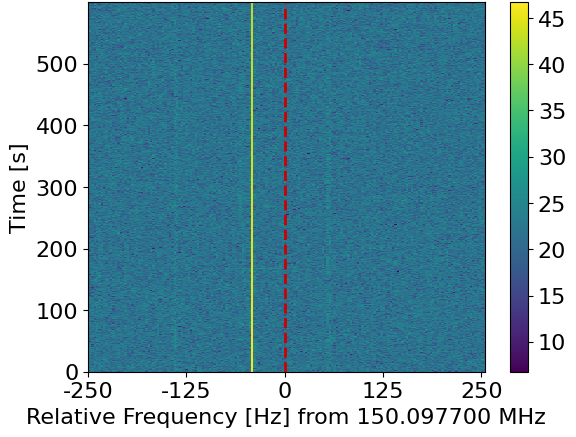
\includegraphics[width=\columnwidth]{B2217+47_crop.png}
    \caption[Narrowband signal detected using REALTA and the \texttt{turboSETI} algorithm.]{Narrowband signal detected using REALTA and the \texttt{turboSETI} algorithm. Dynamic spectra of an example narrowband signal detected in an observation pointing toward PSR B2217+47 using \texttt{turboSETI} with the BL nodes in REALTA. The colour bar shows intensity in arbitrary units while the red dotted line shows a relative frequency of 0~Hz from 150.0977~MHz. The signal does not show any drifting and thus likely has a terrestrial origin.}
    \label{fig:BL_fig}
\end{figure}
%the level of density fluctuations in the solar corona is the major cause of the scattering of radio waves, resulting in large source sizes. However, because of its inherently lower spatial resolution, the magnitude of $\varepsilon$ may be smaller than previously derived in comparison to observations of radio wave scattering in tied-array images. This work was published in \textit{Astronomy and Astrophysics} as \cite{Murphy2021}.

\subsection{Observing Radio Bursts at the Highest Spatial Resolutions.}
The second objective of this thesis was to determine if the size of previously observed type IIIb radio bursts was due to an effect of tied array imaging or radio wave scattering in the corona. 
This is important in determining whether or not the large source sizes of radio bursts have a physical origin or are simply due to a lack of spatial resolution. 
In Chapter \ref{chap:measuring_source_sizes} I described a new method for determining the size of a type IIIb burst directly from interferometric visibilities recorded with LOFAR. This method removes reduces the uncertainty of measured source sizes and removes any ambiguity from imaging deconvolution algorithms.
This was utilised for the first time in the context of solar observations with LOFAR to determined the size of a type IIIb burst. For a burst at 34.76~MHz, the full width at half maximum height (FWHM) along the major and minor axes was found to be 18.8~arcmin~$\pm~0.1$~arcmin and 10.2~arcmin~$\pm~0.1$~arcmin respectively at a plane of sky heliocentric distance of 1.75~R$_\odot$. The expected size of a burst at this frequency, based on the relationship between the spectral width of the striation and spatial extent of emission, was calculated to be 3.18~arcsec. It is important to note that this source size is only an estimate of the vertical extent of the emitting region and as such the actual observed source may be larger due to projection effects. The discrepancy between these two values was investigated and the results suggest that the large size observed is due to radio wave scattering. One further implication of this work is that values of the relative root mean squared density fluctuations $\varepsilon$ which are determined \textit{only} from tied array observations of radio bursts run the risk of over estimating the true value as the effect of imaging on source size has not been fully investigated. This work was published in \textit{Astronomy and Astrophysics} as \cite{Murphy2021}. 

\subsection{Comparing Observations of Radio Bursts to Computational Simulations.}
The final objective of this thesis was to determine if observations of scattered sources matched the predictions of computational simulations. This was achieved by comparing a number of observations of type III bursts to simulations of radio scattering in the solar corona.
Using the new method for determining radio burst size from interferometric visibilities, the spatial properties of 29 type III radio bursts were found. The results of this analysis, comparing the similarities and discrepancies between the observations and computation scatting, are presented in Chapter \ref{chap:observations_vs_theory}.% discusses the measured similarities and discrepancies between these observations and computer simulations of scattering. 
It was found that bursts did not show the change in aspect ratio with respect to heliocentric angle as would be expected following from \cite{Kontar2019}. There are two possible explanations for this, the first being the level of anisotropy is lower than initially suggested by \cite{Kontar2019}. This is supported by an investigation of the parameter space of the scattering simulations by \cite{Zhang2021}. The other is that type III bursts have an intrinsic source size greater than the size of a point source due to scattering. This work favours the latter explanation although it is possible that both can be true. This work suggests that state-of-the-art scattering simulations still do not accurately describe all observed properties of type III radio bursts. In order to use observations of solar bursts at low radio frequencies to determine the turbulent nature of coronal plasma, these discrepancies must be rectified. This work is \textit{in prep} for a scientific publication.
 %Regardless, more must be done to align the theory and simulations with observations.
%theories of scattering are unable to account for the distribution of radio burst source sizes if they are intrinsically point sources. The more likely case is that type III radio bursts have an inherent source size larger than the size due to scattering for a point source.

\section{Future Work}
The research outlined in this thesis has furthered our knowledge of the nature of electron density fluctuations in the solar corona. Direct visibility measurements of the source size of a type IIIb burst has confirmed that density fluctuations are the main cause of large source sizes in observations and not the imaging method used. The work in this thesis has also highlighted discrepancies between observations of type III bursts and scattering simulations. Results from scattering simulations that use values of the relative root mean squared density fluctuations and degree of anisotropy in the power spectrum of fluctuations to match typical observations \citep[e.g.][]{Kontar2017} are not observed in a sample of 29 type III bursts.
%of the inherent source sizes of type III radio bursts and propagation effects due radio wave scattering. 
This work has produced a computationally and conceptually simple method to determine the size and position of a radio burst from its interferometric visibilities. Not only this but, the development of REALTA throughout this PhD allows for the recording of the raw complex voltages from I-LOFAR to study solar radio bursts. I address some open questions that remain and the possibility of future work which builds upon the research presented in this thesis below.
%First, I discuss how data from the TBBs can be utilised to produce dynamic spectra with a temporal resolution of 5~ns. Next, I describe how machine learning techniques can be used to automatically detect a radio burst in real time and how this can lower the data storage requirements of solar radio data on REALTA. I then address the need for a interferometric calibration and imaging pipeline specific to solar radio bursts. Finally, I discuss how a statistical analysis of type IIIb bursts could be useful to quantify radio wave scattering in the corona. 
%As described in \ref{chape:realta}, implementing and algorithm on REALTA to automatically determine when a radio burst has occurred will greatly simplify and reduce the data storage necessary for solar radio observations.
% in order to save on the ever growing data storage issue. Also, REALTA can be adapted to record data from I-LOFAR's TBBs which can record 5~s of data at the 200/160~MHz sampling of I-LOFAR to give the highest temporal resolution of the Sun recorded to date. 

\subsection{On the Future Development of REALTA}
\label{sec:realta_future_work}

Here I have described the hardware for REALTA and given an overview of the software used to record and analyse data recorded from I-LOFAR. First observations of solar radio bursts were showcased, while the broad range of objects that I-LOFAR and REALTA can observe can be seen in \cite{Murphy2021b}. 

LOFAR 2.0 is a series of hardware and software upgrades to the ILT, which will be implemented in a number of stages over the coming years. An upgrade to an international LOFAR station, such as I-LOFAR, will require new receiver units (RCU2), new station beamformers (Station Digital Processors) based on the Uniboard$^2$ architecture \citep{Schoonderbeek2019} and new power, clock and control board for improved station control. The upgrade will greatly improve the instantaneous bandwidth, sensitivity and RFI rejection of an international station.

%The ability to observe using both the LBAs and HBAs simultaneously effectively doubles the data rate of a LOFAR station ($\sim 6.4$~Gbps) and will require a sufficiently high speed network and recording system to record the raw data.
%Two major upgrades to LOFAR are \textbf{due to be completed} in the coming years, namely, LOFAR2.0 \textbf{stage 1}\footnote{\hyperref[LOFAR2.0]{https://www.glowconsortium.de/index.php/en/lofar-about/lofar-2-0}} and Space Weather (LOFAR4SW\footnote{\hyperref[LOFAR4SW]{https://www.lofar4sw.eu}}). The LOFAR2.0 \textbf{stage 1 } upgrade is a major hardware and software upgrade to LOFAR's station electronics including the receiver units and digital processing systems. A LOFAR2.0 station will be able to observe using both the LBAs and HBAs simultaneously, significantly increasing the data output of an international LOFAR station. For upgraded international stations, the increased data rate necessitates a dedicated telescope backend such as REALTA to capture and pre-process the raw voltages in stand-alone mode. 

LOFAR for Space Weather (LOFAR4SW) \footnote{\hyperref[LOFAR4SW]{http://www.lofar4sw.eu}} is a proposed upgrade to LOFAR, currently being designed to enable regular space weather monitoring. If completed, LOFAR4SW would allow near-real-time monitoring of space weather phenomena such as solar flares and coronal mass ejections, interplanetary scintillation and ionospheric disturbances \citep{Carley2020}. This is useful not only to space weather researchers but to the radio astronomy community as a whole as it will broaden our understanding of how space weather can effect the propagation of radio waves in the inner heliosphere and disturbances in the ionosphere and the effect this has on observing astronomical sources. In order to record the data streams from a LOFAR4SW-enabled international station in local mode, a backend such as REALTA will be required to capture the data-stream and to process the raw data so that it can be used by space weather researchers and forecasters. The effectiveness of machine learning algorithms to detect solar radio bursts with REALTA is currently being investigated.

In the future, REALTA will be upgraded to fully include the BL headnode into the system. In order to achieve this, additional VLAN fibre connections will be set up between the UCC compute nodes and the BL headnode and compute nodes. Activating these VLAN fibre connections will allow each machine to record one lane of data and perform real-time channelisation and dedispersion making use of their GPUs.  The BL headnode will distribute an identical OS to the UCC and BL compute nodes and control them in parallel. This will allow REALTA to monitor for radio transients such as those important to SETI research. Upgrades to the data preparation and processing stages of the REALTA data flow (Figure \ref{fig:REALTA_future}) will see REALTA operating fully in real-time (see section \ref{sec:future_software}). %In addition, we are working with Kx Systems developers to create a next-generation system that harnesses the power of kdb+, the fastest time--series database for rapid, real-time data ingestion and processing \footnote{\hyperref[Kx] https://kx.com/blog/dias-kx-and-i-lofar-new-windows-on-the-universe-through-software/}.  

\subsection{On Observing Radio Bursts with TBBs.}
One of the greatest unexplored potentials of solar radio astronomy is extremely high temporal variability of radio bursts. The LOFAR TBBs are capable of recording 5 seconds of raw sampled data from the antennas at 5~ns temporal resolution. The TBBs are an extremely powerful tool that allow one to recreate the LOFAR data processing pipeline entirely in software. Typically, the TBB buffer is frozen before all the data is read out to an external disk. This process is much slower than the 3.2 Gbps recording of RSP data and can take upwards of 40 minutes to read out 5~s of data from every TBB. Over the period September 2017 to March 2018 a method of continually reading from the TBBs in almost real-time was investigated. I assisted in the development of this system and managed to record TBB data on a number of occasions. The data recorded during this time coincided with the solar minimum of solar cycle 24. Radio bursts occurred only once every few months and as such any data taken was essentially noise. Figure \ref{fig:TBB_timeseries} shows 10 ms of noise recorded by the TBBs from LBA number 3 at I-LOFAR.
Throughout my PhD the development of REALTA to record RSP data was a priority and as such, the possibility of a real-time readout of TBBs was not fully explored. 

%
%\begin{figure}[ht]
%\centering
%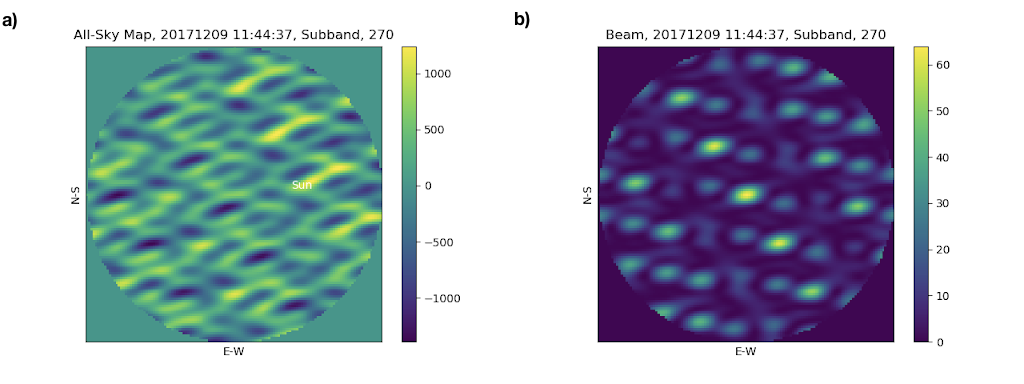
\includegraphics[width=\columnwidth]{AllSky_psf.png}
%\caption[An all sky image made with data from the TBBs at I-LOFAR]{a) An all sky image made with data from the TBBs at I-LOFAR at 52.73~MHz. b) The psf of the antennas for which TBB data was available.}
%\label{fig:TBB_allsky}
%\end{figure}
\begin{figure}[ht]
\centering
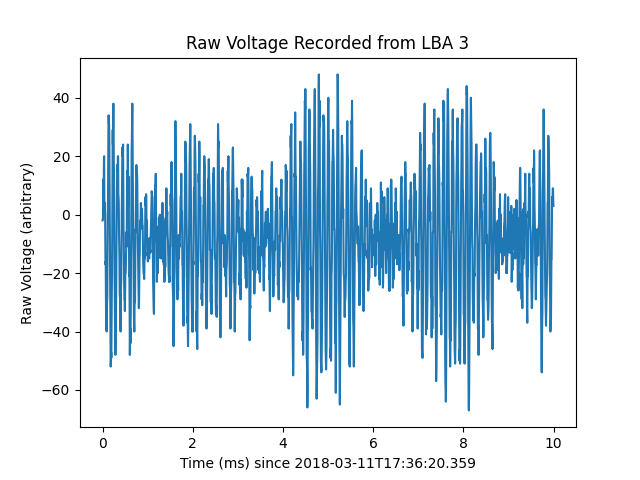
\includegraphics[width=\columnwidth]{TBBtimeseries.png}
\caption[10 ms of data recorded with TBBs from I-LOFAR.]{10 ms of data recorded with TBBs from I-LOFAR, the data presented here is from LBA 3. The beating pattern is likely due to RFI.}
\label{fig:TBB_timeseries}
\end{figure}

TBB data gives one the freedom to recreate a radio telescope entirely in software. It also allows for some unique and ingenuitive signal processing steps. For example, the polyphase filter bank in an RSP takes 1024 time samples before performing a Fourier transform to obtain 512 subbands. This results in a dynamic spectrum with a temporal resolution of 5.12~$\mu$s and 195.3~kHz spectral resolution. Using TBB data it is possible to, instead, perform an FFT on the entire time series, window the resulting spectrum with any desired frequency resolution and inverse FFT each to get a dynamic spectrum with 5~ns temporal resolution and the chosen spectral resolution. 

\begin{figure}[ht]
\centering
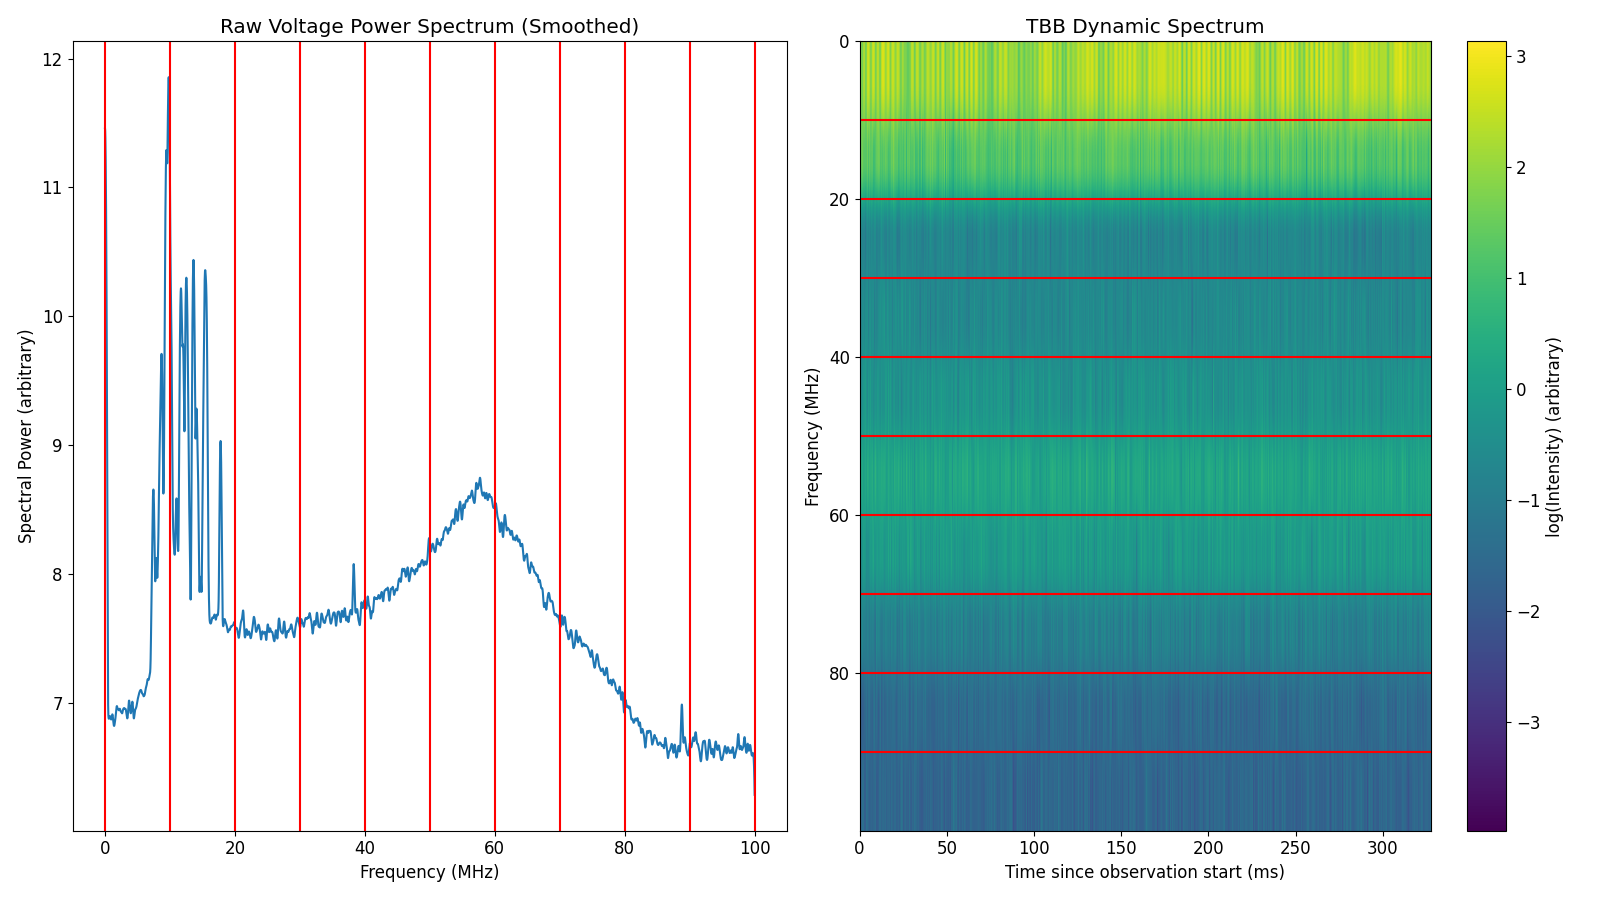
\includegraphics[width=\columnwidth]{TBB_dynamic_spectrum_power_spectrum.png}
\caption[A dynamic spectrum generated with TBB data from I-LOFAR.]{An example of creating a dynamic spectrum from TBB data. The left panel shows the (smoothed) power spectrum of an LBA. The vertical red lines mark the chosen subband edges. The right panel is a dynamic spectrum with a time resolution of 5ns and frequency resolution of $\sim 10$~MHz as determined by the chosen number of subbands, whose edges are shown by the red horizontal lines.}
\label{fig:TBB_dynamicspectrum}
\end{figure}

This is implemented on the same TBB data as shown in Figure \ref{fig:TBB_timeseries} to create the dynamic spectrum shown in Figure \ref{fig:TBB_dynamicspectrum}. The left panel shows the (smoothed) power spectrum of the time series with a number of vertical red lines which indicate the edges of chosen subbands. By performing an inverse Fourier transform on each subband, a dynamic spectrum with a temporal resolution of 5~ns can be created, shown in the right panel. Here, again, the red lines indicate the subband edges. Care must be taken to avoid spectral leakage between subbands. A common approach in avoiding this problem is to apply a window function to each subband. Because the subbands in Figure \ref{fig:TBB_dynamicspectrum} are wide and the data is mostly noise, rectangular windows are appropriate in this case.
 
The ability to record dynamic spectra and retain the 5~ns temporal resolution of the raw LOFAR sampling means that, should they exist, extremely short duration pulsations in solar radio bursts could be studied. These timescales have been completely unexplored to date and offer an exciting chance to push the forefront of solar radio astronomy. Observations at these timescales would allow for the search for fine temporal structure in radio bursts. Because the decay time of radio bursts is attributed to scattering \citep{Krupar2020}, it is likely that any inherent fine temporal structure will get ``blurred out" before being observed. However, there has been no report in scientific literature of solar radio emission at this time scale and thus any such study opens the door into the domain of nanosecond observations of the Sun.

\subsection{On the Automatic Classification of Radio Bursts.}
One of the big challenges facing radio astronomy is the vast amounts of data produced during observations. I-LOFAR produces 3.2 gigabits of data per second meaning that a 5 hour observation can reach sizes of $\sim 7$~TB. As such, observing the Sun for long durations and saving the entire raw dataset regardless of whether a radio burst occurred or not is impractical. An ideal solution would be to automatically determine if a burst has occurred before choosing to save data to disk. 
This is an ideal task for a machine learning (ML) algorithm, which are most commonly used for automatic classification. ML algorithms take thousands to billions of inputs which have been labelled in order to ``learn" how to classify them. The classic example of ML automatic recognition is recognising handwritten numbers from the Modified National Institute of Standards and Technology database \citep[MNIST;][]{LeCun1998}.
\cite{Scully2021} recently showed promising results of using a particular ML algorithm, a convolutional neural network (CNN), to automatically detect and characterise type III radio bursts. They implement the YOLOv2 \citep[You Only Look Once;][]{Yolo9000} algorithm to detect type III bursts and place a bounding box that covers their time and frequency span. Figure \ref{fig:yolo} shows a dynamic spectrum with (left panel) and without (right panel) the intensity inverted and the bounding boxes detected by the CNN. Using a training dataset of simulated type III bursts, the algorithm was able to achieve an accuracy of 82.63$\%$ and can run on data in real-time.  

\begin{figure}[ht]
\centering
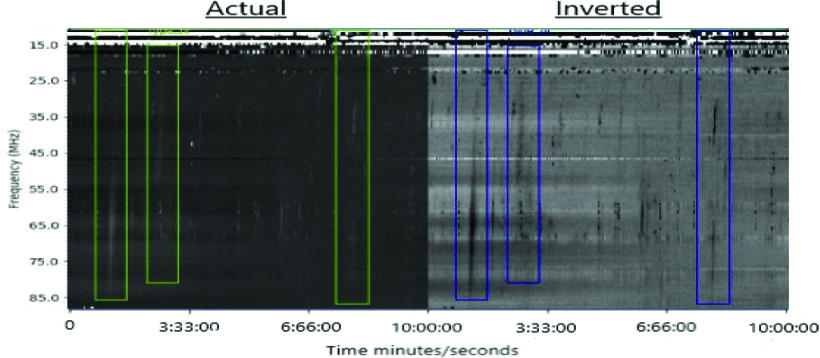
\includegraphics[width=\columnwidth]{scully_yolo.png}
\caption[Automatically detected type III bursts using YOLO.]{Automatically detected type III bursts using YOLO from \cite{Scully2021}. Coloured boxes mark the regions detected by the algorithm to contain a type III burst. The colour bar has been inverted in the right panel in order to better display the type III bursts.}
\label{fig:yolo}
\end{figure}

Implementing this algorithm on REALTA and I-LOFAR would be an ideal test case on real data in real-time, especially as we enter into the next solar cycle. Not only this, but, a detection from the algorithm could be used to trigger a readout of the TBBs.
In their conclusions, \cite{Scully2021} outline some future developments that could improve their results. In particular, a more physical model of type III emission is necessary, rather than the simple morphological model presently used. There is approximately 20~TB of archival data recorded with REALTA many of which contain solar radio bursts. This data, along with simulated dynamic spectra, would provide an ideal training and test set which could improve the performance of the algorithm for I-LOFAR data. The use of ML algorithms in radio data analysis will become all the more important with the next generation of radio telescopes such as the SKA which are expected to drastically increase data rates.

%\subsection{On the Calibration and Interferometric Imaging of Solar Radio Bursts.}
%Interferometric visibilities require calibration in order to account for the effects of the ionosphere. For LOFAR data this is performed using the Default Pre-Processing Pipeline \citep[DPPP;][]{VanDiepen2018}. An observation is made of a known calibrator source for which there is a set of model visibilities. The DPPP calibration algorithm aims to minimise the following equation
%\begin{equation}
%\label{eq:gain}
%\vert \vert \mathbf{V}_{pq} - \mathbf{G}_p \mathbf{M}_{pq} \mathbf{G}^\dag_q \vert \vert
%\end{equation}
%for each baseline $pq$. Here $\mathbf{V}$ are the measured visibilities, $\mathbf{M}$ are the modelled visibilities and $\mathbf{G}$ are known as the gain matrices for each antenna $p$, $q$ and the superscript $\dag$ indicates the Hermitian conjugate. Calibration is done under the assumption of time invariability of the calibrator source. Unfortunately, if the calibrator is close enough to the Sun so that it can be seen in the sidelobes, during bursty periods such as solar radio noise storms this assumption breaks down. Calibration solutions found during these periods are inaccurate at best. The image in Figure \ref{fig:bad_cal} was made with a bad calibration solution and as such, multiple sources can be seen.
%
%\begin{figure}[ht]
%\centering
%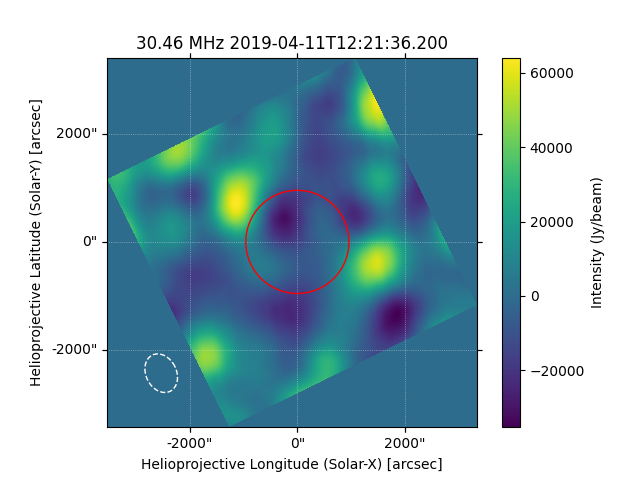
\includegraphics[width=\columnwidth]{2019-04-11T12:21:36-image.png}
%\caption[An example of a solar radio burst imaged with poor calibration.]{A solar radio burst imaged with poor calibration. The colourbar shows intensity in units of Jy/beam. The red circle indicates the solar limb while the dashed white ellipse is the CLEAN beam.}
%\label{fig:bad_cal}
%\end{figure}
%
%Calibration is arguably the most important step in the data processing of interferometric observations. To date, direction dependent calibration on LOFAR solar observations is not a common step taken, despite its proven success in astrophysical observations \citep{DeGasperin2019}. A method to correct for radio bursts in calibration solutions and combine this with direction dependent calibration should be developed  and self-calibration techniques developed for solar imaging with the Murchison Widefield Array \citep[MWA;][]{Mondal2019} should be implemented before the parameter space for imaging algorithms can be fully explored. 
%
%Imaging algorithms such as CLEAN have proven themselves to be widely successful in the field of radio astronomy. However, the ability to produce different results with the same data by only changing the parameters of the algorithm is too subjective when the main focus of one's research is to determine the size of a radio burst. A number of parameters are necessary to run the CLEAN algorithm with number of iterations and weighting scheme having the most notable effect on the output image. Figure \ref{fig:briggs_comparison} shows how changing the Briggs robustness parameter for weighting the visibilites \citep{Briggs1995} affects the resulting image. The top panel shows the results for the CLEAN algorithm implemented in WSCLEAN and the bottom panel shows the results when using multiscale cleaning \citep{Offringa2017}. 
%
%\begin{figure}[ht]
%\centering
%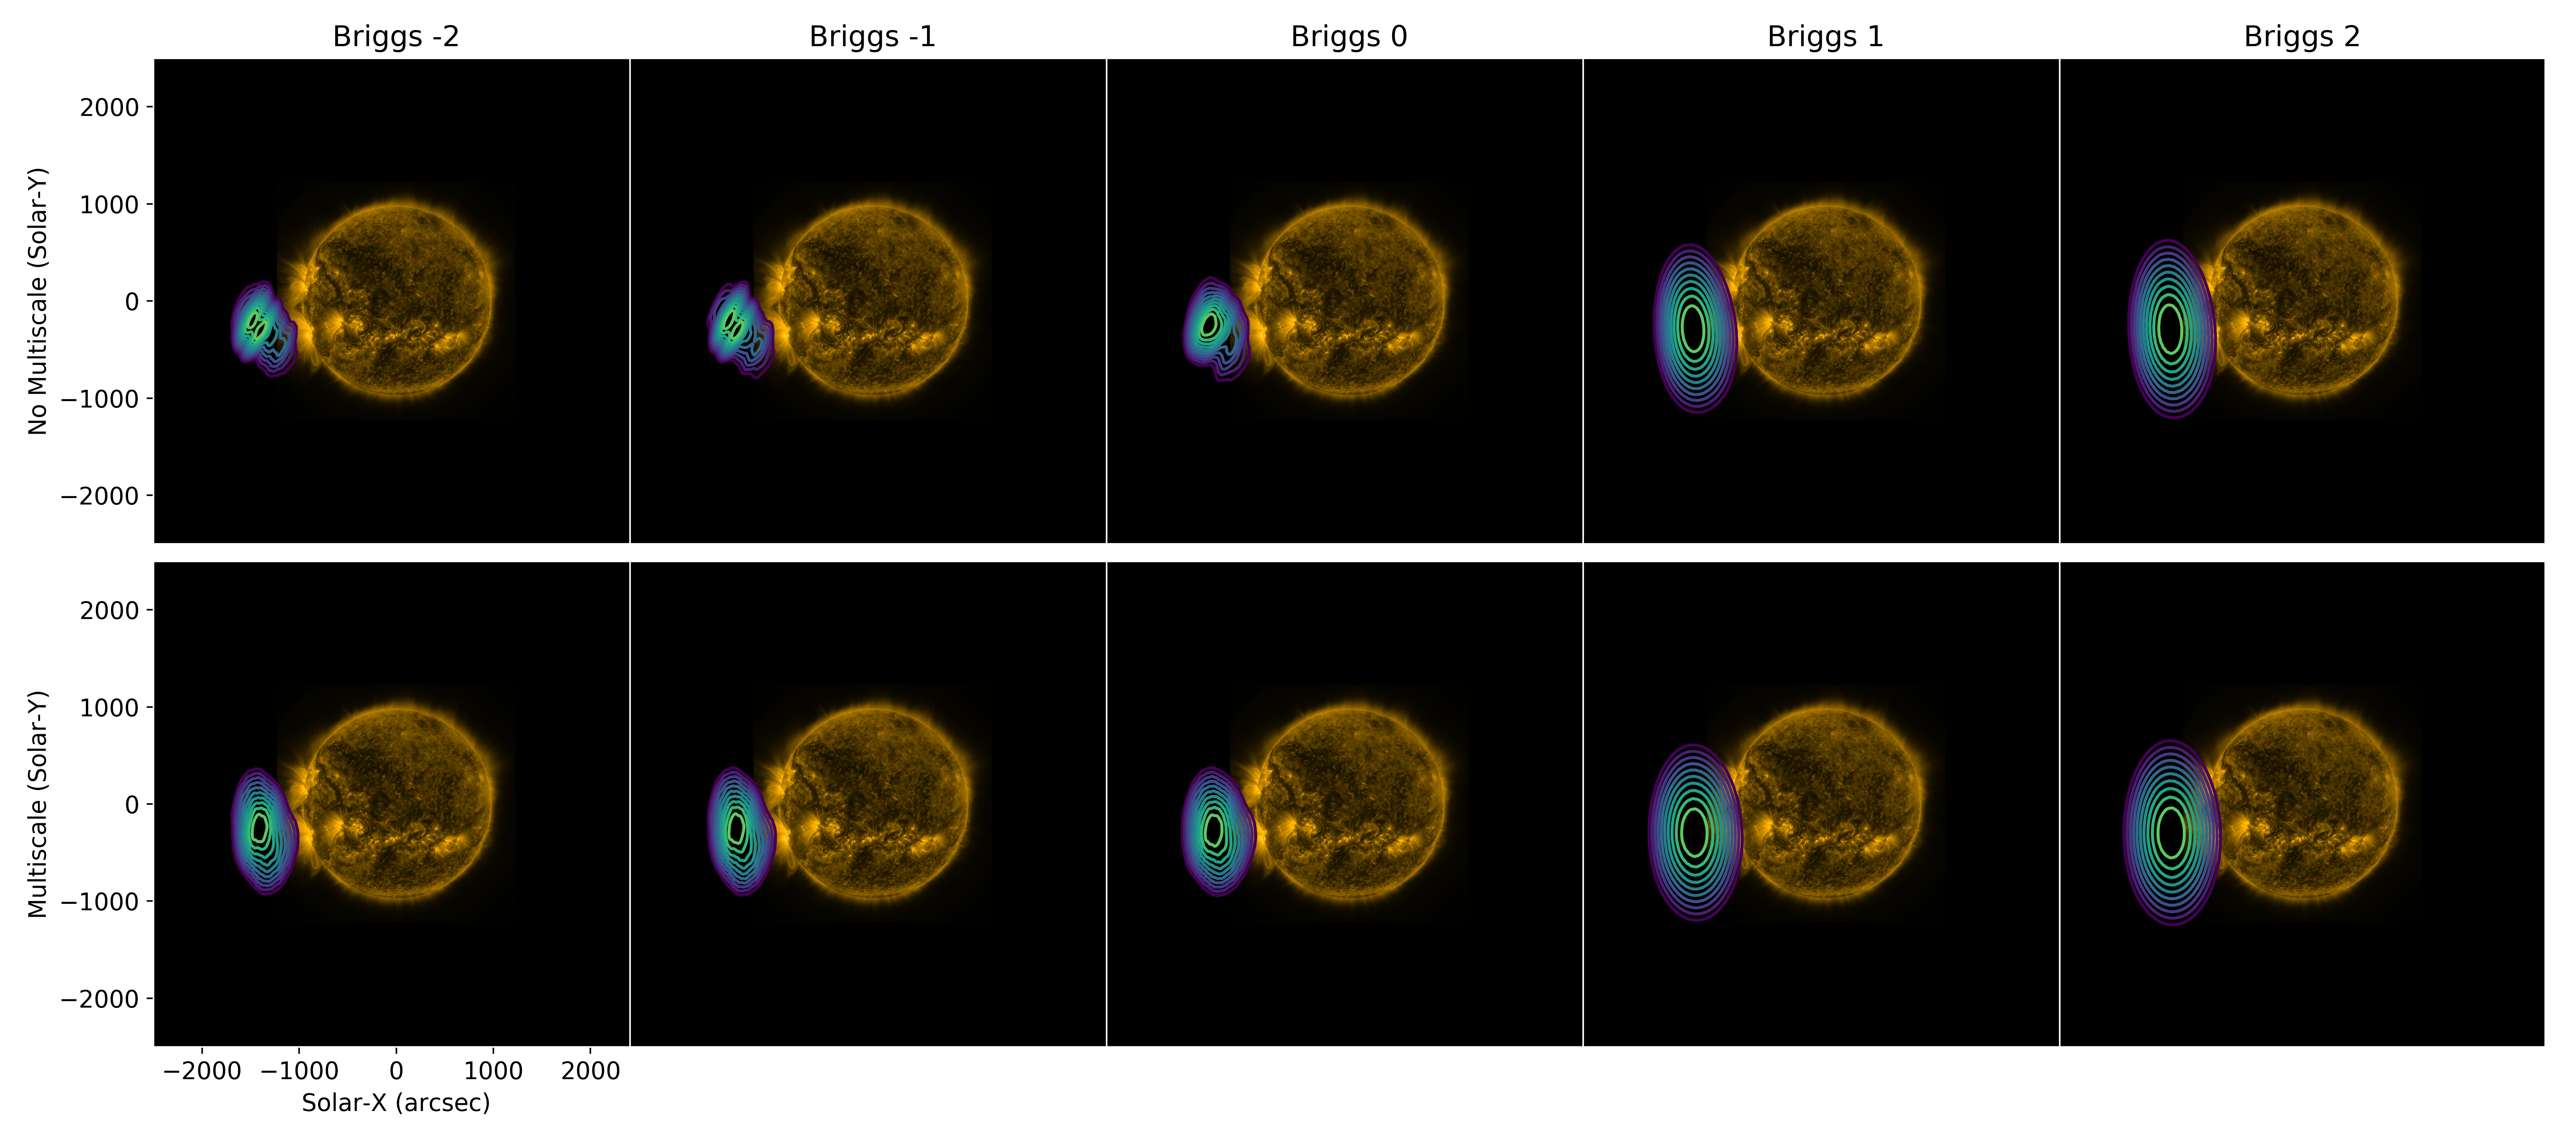
\includegraphics[width=\columnwidth]{briggs_comparison.png}
%\caption[An example of the same solar radio burst imaged with different weighting parameters.]{A solar radio burst imaged multiple times changing the Briggs robustness parameter with (bottom) and without (top) multiscale cleaning.}
%\label{fig:briggs_comparison}
%\end{figure}
%
%In order to consistently image the Sun it is important to determine an appropriate calibration procedure as well as standardise which parameters are to be used in imaging algorithms. Currently, there is little in the way of consensus as to how interferometric solar imaging should be done. \cite{Maguire2021} and \cite{Ryan2021} show interferometric imaging of a radio burst and the quiet radio Sun respectively using LOFAR. Their methodology is broadly similar however, was only finalised after multiple trial and error attempts. Unlike wide-field imaging or other astrophysical sources which can build upon years of research using aperture synthesis techniques, the Sun is a time dependent source and does not enjoy the legacy software that has been developed for other radio astronomy applications. 
%
%In order to extract the most scientific value from current observations, the parameter space for the CLEAN algorithm needs to be explored to avoid making images to a subjective standard. A good start to this work would be to compare how well the algorithm can recreate a known model within the parameter space. The use of supercomputing facilities will be crucial for this to take any reasonable amount of time. 



\subsection{On the Comparisons of Type IIIb Burst Observations and Simulations.}
Type IIIb radio bursts are a subset of type III bursts that exhibit fine spectral features called striae or striations, see Section \ref{sec:typeIII}. The origin of these striations has not been conclusively determined. An early theory by \cite{Takakura1975} suggests that they are due to an electron beam passing through overdense regions in the solar corona. Recently, \cite{Reid2021} presented simulations and observations of type IIIb radio bursts where they have determined how the striae fine structure is developed. Beam driven Langmuir wave modulation by turbulence in the solar corona and the spatial motion of these Langmuir waves due to a non-zero group velocity are both necessary in order to match simulations to observed dynamic spectra and account for individual striation frequency width and duration.

%Figure \ref{fig:reid_stria} shows an individual striation for both a simulated and observed dynamic spectrum. %power density spectra for a number of type IIIb bursts with various background coronas.
%
%\begin{figure}[ht]
%\centering
%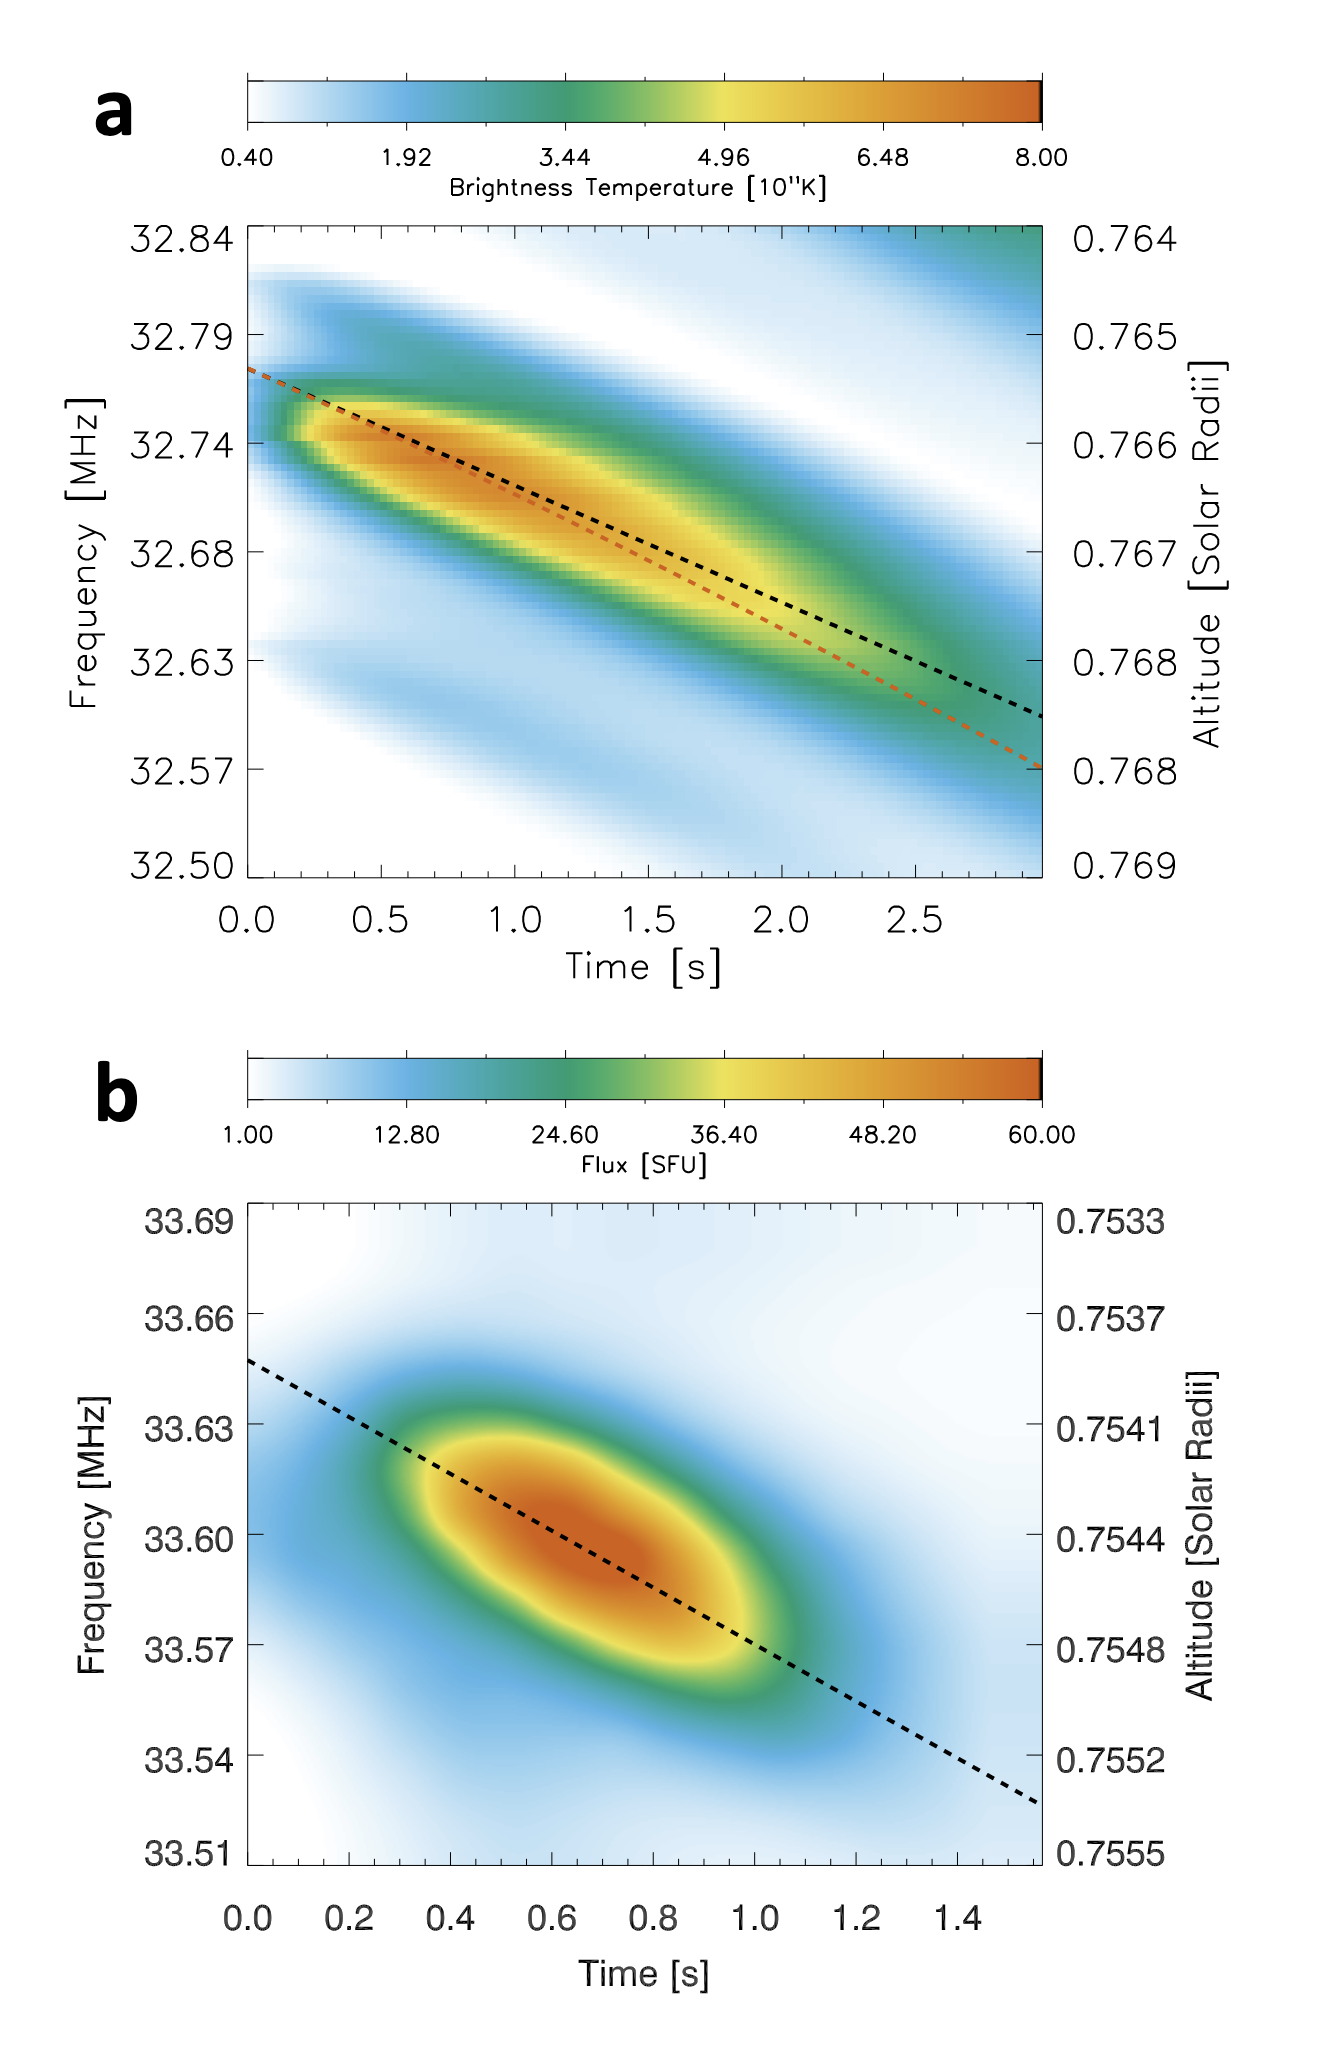
\includegraphics[width=0.5\columnwidth]{reid2021_stria.png}
%\caption[Simulated and observed type IIIb stria by \cite{Reid2021}]{Simulated and observed type IIIb stria by \cite{Reid2021}. Panel a shows an individual stria from a simulated dynamic spectrum with a background temperature of 1~MK. The black dashed line is a linear fit and gives a stria velocity of 0.6~Mm s$^{-1}$ whereas the red dashed line is a quadratic fit with an initial velocity of 0.63~Mm s$^{-1}$ and a final velocity of 0.76~Mm s$^{-1}$. Panel b shows an individual stria from the type IIIb burst on 16 April 2015. The black dashed line is a linear fit with a velocity of 0.69~Mm s$^{-1}$.}
%\label{fig:reid_stria}
%\end{figure}
%
%\begin{figure}[ht]
%\centering
%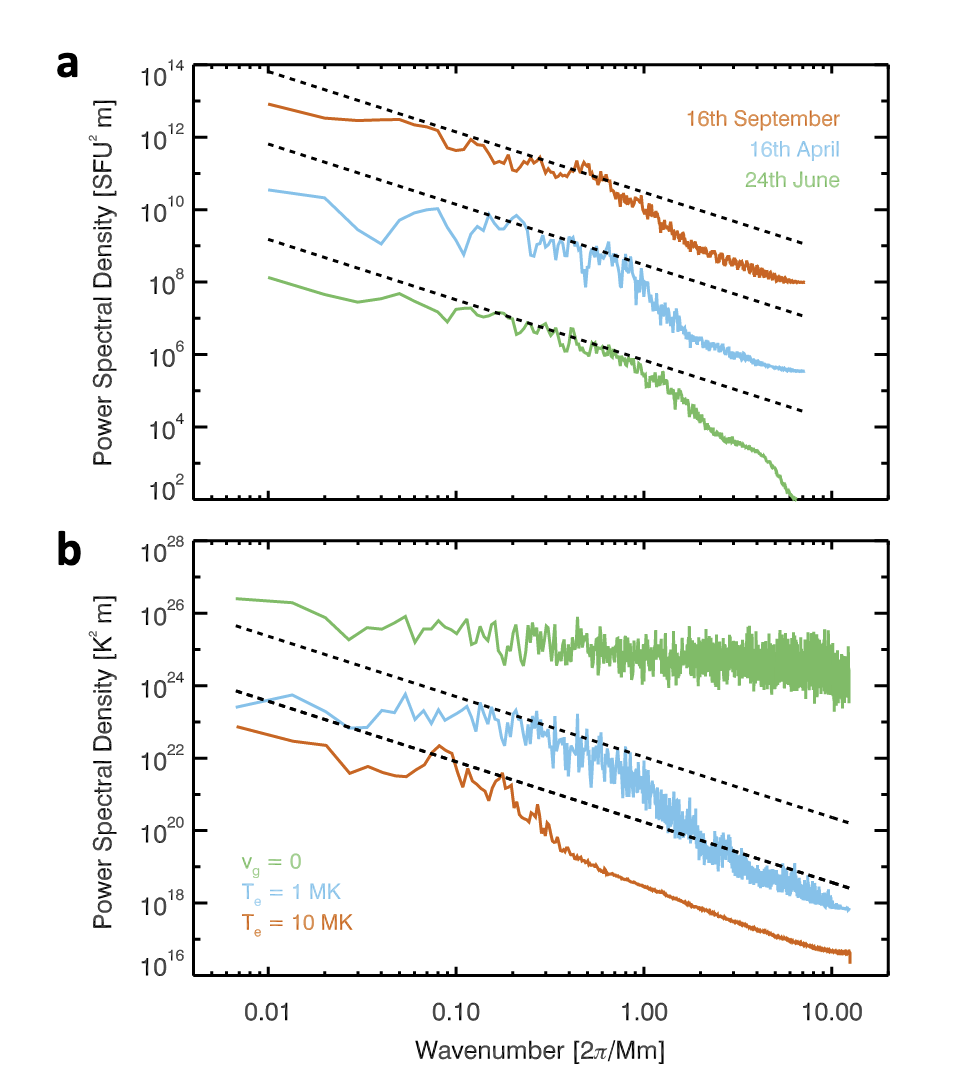
\includegraphics[width=0.75\columnwidth]{reid2021_powerdensityspectra.png}
%\caption[Power density spectrum of observed and simulated type IIIb bursts by \cite{Reid2021}]{Power density spectrum of observed and simulated type IIIb bursts by \cite{Reid2021}. Panel a shows power density spectra for type IIIb bursts observed with LOFAR on 16 September 2015 (red), 16 April 2015 (blue) and 24 June 2015 (green). Panel b shows the power density spectra for simulated type IIIb bursts with a background corona temperature of 1 MK (blue), 10 MK (red) and without a group velocity (green). The dashed balck lines indicate a power law of -5/3, consistent with a Kolmogorov description of turbulence.}
%\label{fig:reid_pds}
%\end{figure}
Following the results from this thesis, the effect radio wave scattering has on the size of type III bursts does not fully agree with scattering simulations (Chapter \ref{chap:observations_vs_theory}). As such, more work is necessary to determine the probable causes of this discrepancy. One possible avenue of investigation would be to perform a similar analysis to Chapter \ref{chap:observations_vs_theory} for type IIIb bursts. By using Equation 1 in \cite{Reid2021}, it would be possible to obtain a value of $\varepsilon$ directly from the dynamic spectrum of a type IIIb burst. Coupling this together with the burst size would give a more qualitative comparison to scattering simulations than has been done previously. Figure \ref{fig:reid_peakflux} shows the peak flux of an observed type IIIb burst on 16 September 2015. The green curve shows the smoothed flux which is used to determine $\Delta I/I$ which can be used to infer a value for $\varepsilon$ from Equation 1 of \cite{Reid2021} repeated here

\begin{equation}
\varepsilon = \frac{\langle\Delta n^2\rangle}{n^2} = \left(\frac{v^2_{Th}}{v^2_b}\right)^2 \frac{\langle \Delta I^2\rangle}{I^2}
\label{eq:RK1}
\end{equation}

\begin{figure}[ht]
\centering
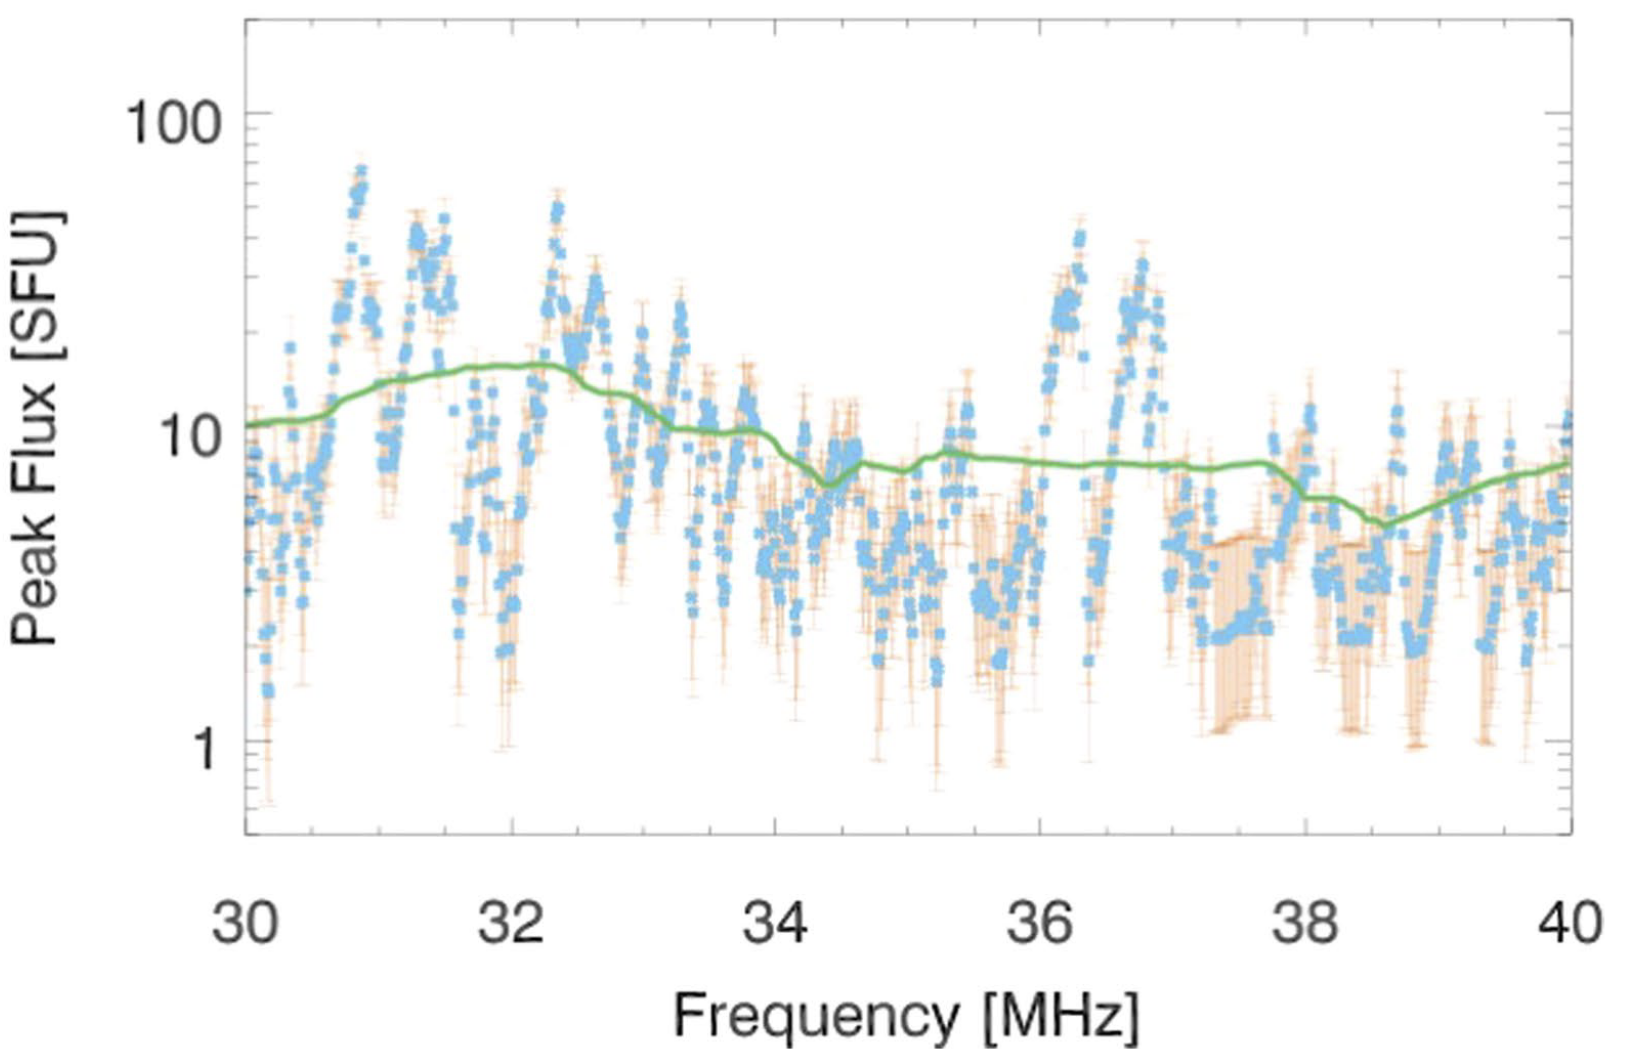
\includegraphics[width=0.75\columnwidth]{reid2021_peak_flux.png}
\caption[Peak flux of a type IIIb burst observed by \cite{Reid2021}.]{Peak flux of a type IIIb burst observed by \cite{Reid2021} on 16 September 2015. The blue points are the actual flux values while the green curve shows a smoothed flux determined using a Savitsky-Golay filter with a characteristic size of 3~MHz. The difference between the peak flux and the smoothed flux is used to calculate $\Delta I/I$ in Equation \ref{eq:RK1}.}
\label{fig:reid_peakflux}
\end{figure}

A previous case study of a type IIIb - III pair (a fundamental-harmonic pair of type III bursts where the fundamental is a type IIIb and the harmonic a type III) was carried out by \cite{Zhang2020}. They found that the fundamental and harmonic emission show different motion as can be seen in Figure \ref{fig:typeIIIbIII} and attribute this to radio wave propagation effects.

\begin{figure}[ht]
\centering
\includegraphics[width=0.7\columnwidth]{Zhang_2020.png}
\caption[Type IIIb - III pair observed by \cite{Zhang2020}.]{A type IIIb - III pair observed by \cite{Zhang2020}. Panels a1-3 show the fundamental type IIIb burst observed with LOFAR and imaged using WSCLEAN. Panels b1-6 show the harmonic type III burst at a frequency of 26.56~MHz.}
\label{fig:typeIIIbIII}
\end{figure}

To date there has been no comparison between a large number of type III and type IIIb bursts where both are emitting at the fundamental plasma frequency using interferometric observations. Applying a technique similar to the visibility fitting described elsewhere in this thesis to determine a characteristic size could be extremely useful in quantifying the level of turbulence necessary to generate type IIIb bursts. This is also an excellent opportunity to use \textit{in-situ} data from Parker Solar Probe \citep[PSP;][]{Fox2016} and Solar Orbiter \citep{Muller2020} to confirm the predictions made with remote measurements from LOFAR and other radio telescopes. 

%\subsection{On the Structure Function of Density Turbulence in the Corona.}
%\cite{Bastian1994} describes the

\section{Concluding Remarks.}
The research presented in this thesis is a study of the low radio frequency Sun at some of the highest temporal, spectral and spatial resolutions to date. Our knowledge of radio wave propagation in the solar corona has been expanded as a result and the potential for further study is great. Using a new method in the context of LOFAR solar observations that I developed, I determined that the large size observed for a type IIIb radio burst is due to radio wave scattering in the corona and that this effect may be over estimated by previous tied array imaging observations of the same. Following from this, I investigated the source size and position of 29 type III bursts using the same method. My conclusion from this is that the level of anisotropy of radio wave scattering is lower than first expected by simulations and that type III bursts have an intrinsic source size of the order of 10 arcmins. Parallel to this, I helped develop and install REALTA at I-LOFAR which has recorded numerous radio noise storms at 5.12~$\mu$s temporal resolution and 195.3~kHz spectral resolution. 

With the upgrade to LOFAR2.0 and other next generation radio telescopes such as the Square Kilometre Array \citep[SKA;][]{McMullin2020} imminent, automatic detection of solar radio bursts will become all the more important. Machine learning algorithms have an important part to play in the automatic detection and classification of solar radio bursts in the near future. Until then, development of solar-specific calibration and imaging techniques can help maximise the quality of observations from modern day interferometers such as LOFAR.  

There are many questions that remain unanswered about radio wave scattering in the corona, the most relevant to this thesis being why do scattering models not fully agree with observations? Recent advancements in the theory of fine structure generation in type IIIb bursts may bridge the gap between observations and simulations.

The work and research undertaken as part of this thesis has improved our understanding of and ability to observe and analyse solar radio emission. By combining the imaging technique developed during this thesis with \textit{in-situ} measurements of coronal plasma, some of the long standing questions in radio wave propagation are bound to be answered. 
%They say science is done incrementally. In that case, this thesis is as incremental as it gets. While I do not claim to have made any ground breaking discoveries, I do truly believe that the work and research undertaken as part of this thesis has improved our understanding of and ability to observe and analyse solar radio emission. I have but marked the path, it is for others to now follow it.	














